\section{Organização}
\qquad A Empresa S.Roque ou ROQ
\emptyline
Localizada no coração do Vale do Ave, a S.Roque - Máquinas e Tecnologia Laser S.A., labora em instalações próprias com uma área coberta de aproximadamente 25.000 $m^{2}$. A empresa orgulha-se de ser hoje uma experiente e bem-sucedida PME, tendo sido distinguida pelo IAPMEI como PME Líder e de Excelência pelo quarto ano consecutivo.
\emptyline
Líder nacional no seu campo de atividade – fabrico de máquinas e equipamentos para as indústrias de estamparia têxtil e embalagem - emprega atualmente mais de 350 funcionários distribuídos pelos seus diferentes departamentos.
\emptyline
Com instalações funcionais e com profissionais qualificados e experientes, a S.Roque dispõe das mais avançadas ferramentas e tecnologias na área da metalomecânica, do design e da elaboração de produto. Os equipamentos fabricados são de conceção própria, desenhados por um departamento técnico altamente especializado para corresponder aos desígnios de projeto e com o objetivo de satisfazer qualitativamente as solicitações do cliente mais exigente.
\emptyline
Hoje, após a conquista e solidificação incontestável da liderança do mercado português, tornando-se num dos líderes mundiais na área da estamparia e da embalagem, a S.Roque produz e comercializa um extenso catálogo com diferentes produtos e trabalha com clientes/parceiros um pouco em todo o mundo: Espanha, França, Itália, Inglaterra, Alemanha, Holanda, Suécia, Romênia, África do Sul, Marrocos, Tunísia, Angola, Turquia, Kuwait, Índia, China, Vietnam, Malásia, Camboja, Rússia, Bulgária, Brasil, Argentina, Peru, Colômbia, Honduras, El Salvador e E.U.A.
\begin{figure}[ht]
\begin{center}
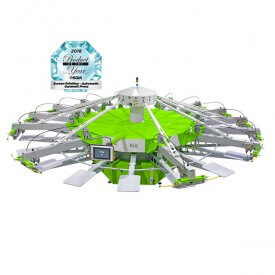
\includegraphics[scale=0.5]{./image/ROQ/maquinas/ECO-P18_600x600-2-275x275.jpg}
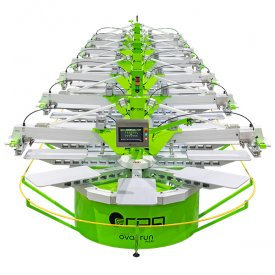
\includegraphics[scale=0.5]{./image/ROQ/maquinas/EVO-600x600-275x275.jpg}
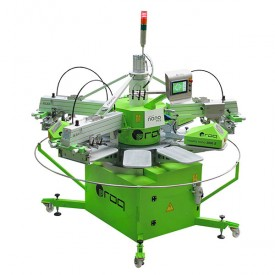
\includegraphics[scale=0.5]{./image/ROQ/maquinas/nanop10-275x275.jpg}
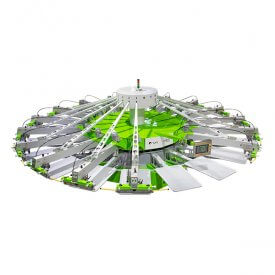
\includegraphics[scale=0.5]{./image/ROQ/maquinas/NEXTP18-600x6001-275x275.jpg}
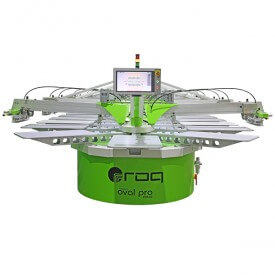
\includegraphics[scale=0.5]{./image/ROQ/maquinas/PRO-600x600-275x275.jpg}
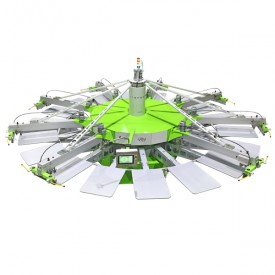
\includegraphics[scale=0.5]{./image/ROQ/maquinas/You-600x600-275x275.jpg}
\end{center}
\caption{Produtos Principais}
\end{figure}
%%%%%%%%%%%%%%%%%%%%%%%%%%%%%%%%%%%%%%%%%%%%%%%%%%%%%%%%%%%%%%%%%%%%%%%%%%%%%%%%%
\newpage
A S.Roque dedica-se à construção e comercialização de máquinas de estamparia têxtil há mais de 30 anos. Embora a sua génese esteja ligada à manutenção destes equipamentos, rapidamente foi identificada a oportunidade de construir de raiz este tipo de máquina. Os têxteis estavam em alta no Vale do Ave, e a S.Roque aproveitou para criar um produto de qualidade para uma clientela extremamente exigente. A empresa não se contentou em servir apenas o seu nicho de mercado, desde muito cedo que procurou a internacionalização. Numa primeira fase e por motivos geográficos criou parecerias europeias, numa segunda fase e por questões culturais dedicou-se ao Brasil e América do Sul. Neste milénio tornou-se numa marca global de referência na área onde atua. Todo e qualquer mercado está ao nosso alcance.\\
Hoje mais do que nunca não chega ter o melhor produto do mercado, é também necessário apresentar um serviço excelente e acessível em qualquer ponto do globo. A S.Roque orgulha-se de procurar a excelência em tudo em que se envolve com especial destaque para a procura de soluções.
\emptyline
Em 2015 a marca S.Roque transformou-se em ROQ. Atendendo às necessidades do século XXI reconhecemos a necessidade de criar uma marca verdadeiramente global que consiga de uma forma eficaz transmitir mais de 30 anos de história, inovação, internacionalização e conhecimento.
%%%%%%%%%%%%%%%%%%%%%%%%%%%%%%%%%%%%%%%%%%%%%%%%%%%%%%%%%%%%%%%%%%%%%%%%%%%%%%%%%
